\documentclass[conference]{IEEEtran}
\renewcommand{\rmdefault}{cmr}
\renewcommand{\sfdefault}{cmss}
\renewcommand{\ttdefault}{cmtt}
\usepackage{amsmath,amssymb,amsfonts}
\usepackage{graphicx}

\def\BibTeX{{\rm B\kern-.05em{\sc i\kern-.025em b}\kern-.08em
    T\kern-.1667em\lower.7ex\hbox{E}\kern-.125emX}}
\begin{document}

\title{Hybrid Event-Driven Spoofing Detection (HEDSD) method Wireless Sensor Networks}

\author{\IEEEauthorblockN{1\textsuperscript{st} Prashanth K}
\IEEEauthorblockA{\textit{Department of Master of Computer Applications} \\
\textit{RV College of Engineering(Affiliated to VTU, Belagavi)}\\
Bengaluru, India \\
prashanthk@rvce.edu.in}
\and
\IEEEauthorblockN{2\textsuperscript{nd} Usha J}
\IEEEauthorblockA{\textit{Department of Master of Computer Applications} \\
\textit{RV College of Engineering(Affiliated to VTU, Belagavi)}\\
Bengaluru, India \\
ushaj@rvce.edu.in}
}
\maketitle

\begin{abstract}
This paper proposes an energy-adaptive hybrid spoofing detection framework for resource-constrained industrial Wireless Sensor Networks (WSNs), addressing the fundamental trade-off between detection accuracy and sensor battery longevity. While continuous public-key cryptographic authentication (ECDSA NIST P-256) guarantees unforgeable origin security, executing signature verification on every packet rapidly exhausts node battery reserves ($90.0$~mJ per check). Conversely, lightweight physical-layer fingerprinting schemes ($5\,\mu\text{J}$) suffer elevated false alarms under industrial channel fading. To resolve this dilemma, the proposed framework introduces a multi-tier decision architecture combining physical-layer spatial RSSI screening, an event-driven trigger mechanism, context-aware dynamic trust scoring ($T = \alpha T_{\text{auth}} + \beta T_{\text{behavior}} + \gamma T_{\text{energy}}$), and an Early Warning Score (EWS) temporal accumulator. Unlike existing approaches relying on continuous monitoring or heavy computational models, our framework selectively activates cryptographic signature audits strictly upon anomaly detection while employing a three-tier energy-adaptive mode switching strategy that gracefully degrades evaluation complexity as battery levels decline. Validated through discrete-event network simulations across a 401-node industrial factory floor processing over 1.1 million telemetry packets, the proposed model selectively triggers heavy cryptographic audits on only $0.53\%$ of incoming traffic, achieving a $99.40\%$ reduction in per-packet evaluation energy (from $90.00$~mJ down to $0.540$~mJ). The framework delivers a $98.18\%$ detection accuracy with an exceptionally low $0.03\%$ false positive rate, preserving $63.4\%$ of cluster head battery capacity and extending network operational lifetime by over 130-fold.
\end{abstract}

\begin{IEEEkeywords}
Wireless Sensor Networks, Identity Spoofing Detection, Physical-Layer Security, Adaptive Trust Management, Resource Minimization, Industrial Internet of Things.
\end{IEEEkeywords}

\section{Introduction}
A spoofing attack in wireless communication networks is a critical security threat where an unauthorized adversary maliciously assumes the identity of a valid device by forging its network credentials or physical-layer transmission signatures~\cite{ref_spoof_survey_07}.
Through deception as a genuine node, the adversary avoids authorization at the periphery, accesses the broadcast wireless channel shared by the network, and communicates unauthorizedly with other nodes or gateways. As a result, the deceiver is able to inject fake measurements, alter the routing decisions made based on those measurements, cause disruption through denial-of-service attacks, and violate the confidentiality and integrity of the entire network~\cite{ref_wsn_threats_06}. Because of the openness of radio waves and the lack of any physical protection for low-power wireless devices, identity spoofing has become one of the most widespread vulnerabilities of modern wireless technologies.

Wireless Sensor Networks (WSNs) constitute the digital infrastructure of the Industrial Internet of Things (IIoT) and facilitate the continuous monitoring of the environment, automation, control, and predictive maintenance in smart factories and critical infrastructures~\cite{ref_iot_survey_01, ref_wsn_ind_02}. In the typical industrial deployment, hundreds of low-power wireless sensor nodes continuously collect the telemetry data (e.g., temperature, vibrations, pressure, and flow rates) and forward packets in multi-hop clustered architectures to a central Base Station (BS) or industrial edge gateway~\cite{ref_cluster_03, ref_iiot_sec_04}.

However, because of the open-broadcast characteristic of wireless channels for communication, no physical tamper resistance in industrial field devices, and the requirement for minimal energy consumption, industrial WSNs become highly susceptible to wireless attacks~\cite{ref_phy_sec_05, ref_wsn_threats_06}. Identity Spoofing attacks and \textbf{Sybil Attacks} represent such security threats. In an identity spoofing attack, the attacker pretends to be a genuine sensor by imitating its MAC address or network layer ID, introducing malicious control signals, corrupting sensor readings, and disrupting routing of the cluster~\cite{ref_spoof_survey_07, ref_sybil_08}. Sybil attacks involve one rogue sensor node claiming different fake sensor IDs at the same time, making it dominant in the cluster head election process and data aggregation procedure~\cite{ref_sybil_wsn_09}.

To protect against origin spoofing, conventional network security frameworks mandate continuous public-key cryptographic signature verification, most notably using Elliptic Curve Cryptography (ECDSA NIST P-256) or HMAC authentication for every transmitted packet~\cite{ref_ecc_wsn_10, ref_crypto_cost_11}. Although continuous cryptographic authentication delivers robust security assurances against identity forgery, it incurs an unsustainable computational and energy tax on resource-constrained sensor hardware~\cite{ref_mcu_energy_12}. Experimental benchmarks on 16-bit MSP430-class sensor microcontrollers~ (operating at 8 MHz) equipped with CC2420 transceivers demonstrate that verifying a single ECDSA-P256 digital signature consumes approximately $90.0$~mJ of electrical energy~\cite{ref_cryptography_io_43} and takes upwards of $1.2$ seconds of processing time~\cite{ref_ecdsa_bench_13, ref_msp430_bench_14}. For Cluster Heads (CHs) processing thousands of telemetry packets per hour, continuous signature verification leads to rapid battery depletion, node premature failure, network partitioning, and catastrophic loss of operational monitoring capacity~\cite{ref_ch_depletion_15}.

Conversely, lightweight non-cryptographic anomaly detection schemes (such as pure Received Signal Strength Indicator (RSSI) fingerprinting or standalone machine learning classifiers) offer micro-joule operational overhead ($5$--$100\,\mu\text{J}$), but suffer from elevated False Positive Rates (FPR) under industrial radio interference, link quality fluctuations~\cite{ref_interference_wsn_29}, multipath fading, and dynamic shadowing effects~\cite{ref_lognormal_shadow_45}. Pure ML models operating in static regimes fail to adapt when physical channel conditions fluctuate or when network energy levels drop, leading to either security breaches or unnecessary alarm generation~\cite{ref_adaptive_trust_18}.

To resolve this critical energy-security trade-off, this paper proposes the \textbf{Hybrid Event-Driven Spoofing Detection (HEDSD)} framework. The proposed model adopts an industrial adaptive decision method, bridging physical-layer radio propagation properties, lightweight machine learning, dynamic multi-factor trust evaluation, and conditional cryptographic verification into a multi-tier defense architecture tailored for large-scale industrial WSNs.

\subsection{Research Motivations and Key Contributions}
The key driver for the work presented here comes from the challenging resource-security trade-off in industrial WSNs, where while continuous public key cryptography-based authentication ensures tamper-proof origination, it drains node battery power significantly (90.0 mJ per authentication), whereas while lightweight physical layer filtering (5 μJ per check) has a high false alarm rate. To overcome this trade-off, this paper introduces a multi-tier hybrid spoofing detection framework that selectively restricts public-key signature verification to verified anomaly events while employing energy-adaptive mode switching as battery reserves decline. The key contributions of this work include: (i) a multi-tier adaptive architecture that integrates physical-layer RSSI screening with conditional ECDSA-P256 signature auditing to minimize steady-state energy consumption; (ii) a context-aware dynamic trust model ($T_i = \alpha T_{\text{auth}} + \beta T_{\text{behavior}} + \gamma T_{\text{energy}}$) featuring threat-driven weight adaptation ($\alpha, \beta, \gamma$) to dynamically balance cryptographic reliance against battery conservation; (iii) a temporal Early Warning Score accumulator ($\text{EWS}_i$) and joint isolation rule to suppress transient fading spikes and eliminate false quarantining ($0.03\%$ FPR); and (iv) extensive discrete-event simulation across a 401-node industrial network validating a $99.40\%$ reduction in per-packet evaluation energy ($0.540$~mJ/pkt), $98.18\%$ spoofing detection accuracy, and a 130-fold operational lifetime extension.

\section{Related Work and Literature Survey}
\label{sec_related_work}

Spoofing attack detection in Wireless Sensor Networks has been widely studied across four primary paradigms: (i) Physical-Layer Radio Fingerprinting, (ii) Cryptographic Origin Authentication, (iii) Trust and Reputation Security Models, and (iv) Machine Learning Anomaly Classifiers.

\subsection{Physical-Layer Radio Fingerprinting}
Physical-layer security approaches leverage inherent physical characteristics of wireless radio propagation, such as Received Signal Strength Indicator (RSSI), Channel State Information (CSI), Phase Difference of Arrival (PDoA), and Angle of Arrival (AoA), to authenticate node origin without relying on secret keys~\cite{ref_phy_sec_05, ref_rssi_finger_19}. 

Yang \textit{et al.}~\cite{ref_yang_rssi_20} proposed K-means clustering over RSSI spatial profiles to detect identity spoofing in IEEE 802.11 networks. Their approach demonstrated that spatial correlation between RSSI readings from different antenna receivers can effectively distinguish legitimate transmissions from spoofed signals originating from distinct spatial locations. However, their model assumed stationary radio channels without heavy industrial multipath fading.

Liu \textit{et al.}~\cite{ref_liu_csi_21} utilized fine-grained CSI amplitude and phase features from OFDM subcarriers to detect spoofing in industrial wireless networks. While CSI provides higher spatial granularity than RSSI, acquiring CSI requires specialized software-defined radio (SDR) hardware or modified Wi-Fi NIC drivers, rendering it impractical for low-cost IEEE 802.15.4 / ZigBee sensor nodes. Furthermore, environmental dynamics such as moving industrial machinery or overhead cranes cause rapid spatial decorrelation, resulting in elevated false positive rates ($>12\%$)~\cite{ref_csi_fading_22}.

\subsection{Cryptographic Origin Authentication Schemes}
Cryptographic approaches guarantee origin authenticity using symmetric MACs or asymmetric digital signatures~\cite{ref_crypto_cost_11}. Heinzelman \textit{et al.}~\cite{ref_leach_sec_23} integrated symmetric key pre-distribution into clustered WSN architectures (SecLEACH). While symmetric HMAC checks incur low computational overhead ($<10\,\mu\text{J}$), key compromise at a single sensor node exposes the entire cluster to impersonation and Sybil attacks.

To prevent master key compromise, public-key cryptographic primitives, specifically Elliptic Curve Cryptography (ECC), have been implemented for WSNs~\cite{ref_ecc_wsn_10}. Public-key schemes like TinyECC~\cite{ref_tinyecc_24} and ECDSA NIST P-256 enable unforgeable per-packet signature generation and verification. However, performance studies by Piotrowski \textit{et al.}~\cite{ref_mcu_energy_12} and Wandeler \textit{et al.}~\cite{ref_msp430_bench_14} proved that verifying an ECDSA-P256 signature on 16-bit sensor microcontrollers (e.g., TI MSP430 or Atmel ATmega128L) requires $90.0$--$120.0$~mJ per packet. In dense industrial telemetry scenarios where cluster heads receive thousands of packets per hour, continuous cryptographic verification causes rapid battery drain, shortening cluster head lifetime to a few days~\cite{ref_ch_depletion_15}.

\subsection{Trust and Reputation Management Systems}
Trust-based security systems evaluate node trustworthiness by monitoring historical communication behaviors, packet forwarding ratios, and sequence number continuity~\cite{ref_adaptive_trust_18, ref_trust_wsn_25}. Ganeriwal \textit{et al.}~\cite{ref_rfsn_26} introduced the Reputation-based Framework for Sensor Networks (RFSN), utilizing Beta reputation distributions to compute trust scores. 

Sun \textit{et al.}~\cite{ref_dynamic_trust_27} developed a multi-attribute dynamic trust model incorporating energy consumption and packet delivery metrics. Similarly, Zhang \textit{et al.}~\cite{ref_trust_sybil_28} applied fuzzy trust logic to isolate Sybil nodes in multi-hop WSNs. Recently, Wang \textit{et al.}~\cite{ref_tmc_trust_2024} (IEEE TMC 2024) proposed a dynamic trust management scheme for malicious node detection in weak-link WSNs, utilizing adaptive behavior observation. However, existing dynamic trust models process every transmitted frame continuously, incurring constant computational overhead regardless of node battery drain or network threat level.

\subsection{Machine Learning-Assisted Anomaly Classifiers}
Recent advances in machine learning (ML) have led to the adoption of supervised and unsupervised anomaly classifiers for WSN intrusion detection~\cite{ref_ml_ids_17, ref_ml_wsn_30, ref_wiley_ids_2024}. Machine learning algorithms, including Support Vector Machines (SVM), Decision Trees (DT), Random Forests (RF), and XGBoost, extract multi-dimensional features (such as packet arrival intervals, RSSI variations, and sequence gaps) to detect spoofing patterns~\cite{ref_rf_wsn_31, ref_xgb_ids_32}.

Zhang \textit{et al.}~\cite{ref_jsen_svm_2022} (IEEE Sensors J. 2022) developed a multi-parameter spoofing detection scheme leveraging Support Vector Machines (SVM) on physical signal parameters. Tan \textit{et al.}~\cite{ref_deep_ids_33} and Vinayakumar \textit{et al.}~\cite{ref_dt_wsn_34} implemented deep neural network (DNN) architectures for intrusion and spoofing detection in IoT networks, achieving $98.5\%$ detection accuracy. Al-Fuhaidi \textit{et al.}~\cite{ref_wiley_ids_2024} evaluated anomaly-based WSN intrusion detection using ensemble classifiers. However, running continuous ML inference on memory-constrained sensor microcontrollers ($<10$ KB RAM) is computationally expensive ($100$--$12,500\,\mu\text{J}$ per packet). Standalone ML classifiers operating without physical spatial verification or selective cryptographic fallback remain vulnerable to adversarial evasion attacks and mimicry spoofing~\cite{ref_adv_ml_35}.

\subsection{Hybrid Trust-ML and Physical-Layer Authentication}
To combine physical signal features with trust logic, Ali \textit{et al.}~\cite{ref_pla_mdpi_2024} proposed a multi-attribute physical-layer authentication (PLA) framework utilizing RSSI, battery levels, and machine learning classifiers. Kumar \textit{et al.}~\cite{ref_iotj_fedtrust_2024} (IEEE IoTJ 2024) introduced a trust-aware authentication scheme combining federated machine learning with behavioral trust scoring. While federated trust models deliver strong security assurances, their high communication overhead and intensive model aggregation cycles make them unsuitable for low-power IEEE 802.15.4 sensor nodes.

\subsection{Literature Summary and Research Gaps}
Existing WSN spoofing detection approaches—spanning physical RSSI/CSI profiling~\cite{ref_yang_rssi_20, ref_liu_csi_21}, continuous ECDSA authentication~\cite{ref_mcu_energy_12}, dynamic trust systems~\cite{ref_tmc_trust_2024}, SVM classifiers~\cite{ref_jsen_svm_2022}, multi-attribute PLA~\cite{ref_pla_mdpi_2024}, federated learning~\cite{ref_iotj_fedtrust_2024}, and ensemble IDS~\cite{ref_wiley_ids_2024}—are indexed across top-tier computer science venues. As summarized in Table~\ref{tab_related_work_comparison}, current techniques either exhibit high sensitivity to industrial channel fading or incur prohibitive computational costs ($0.065$--$90.00$~mJ/pkt) without providing multi-tier adaptive trigger capabilities.

\begin{table*}[t]
\caption{Comparative Taxonomy of State-of-the-Art WSN Spoofing Detection Approaches vs. Proposed HEDSD}
\label{tab_related_work_comparison}
\centering
\small
\resizebox{\textwidth}{!}{%
\begin{tabular}{|l|c|c|l|}
\hline
\textbf{Detection Technique} & \textbf{Overhead (mJ/Pkt)} & \textbf{Adaptive Trigger} & \textbf{Primary Technical Limitation} \\
\hline
Physical RSSI Clustering & $0.005$ mJ & No & Vulnerable to Channel Fading \\
Physical CSI Profiling & $0.080$ mJ & No & Requires Specialized SDR Hardware \\
Continuous ECDSA-P256 & $90.000$ mJ & No & Severe Per-Packet Battery Drain \\
Dynamic Trust Management & $0.065$ mJ & No & Lacks Adaptive Mode Switching \\
SVM Multiparameter Spoofing & $0.450$ mJ & No & High Matrix Computation Overhead \\
Multi-Attribute Physical Auth & $0.120$ mJ & No & Lacks Multi-Factor Trust Engine \\
Federated Trust-ML Auth & $2.500$ mJ & No & Heavy Federated Parameter Sync \\
Anomaly WSN IDS & $0.350$ mJ & No & Lacks Physical Spatial Proof \\
\hline
\textbf{Proposed HEDSD (This Work)} & $\mathbf{0.540}$ \textbf{mJ} & \textbf{Yes (3-Tier)} & \textbf{Optimal Security-Efficiency Balance} \\
\hline
\end{tabular}%
}
\end{table*}

\section{System Model and Industrial Scenario Setup}
\label{sec_system_model}

We model an industrial factory floor ($1000\text{ m} \times 1000\text{ m}$) operating a two-tier clustered Wireless Sensor Network of $N = 401$ nodes, comprising a central line-powered Base Station, $40$ Cluster Heads ($E_{\text{CH}}^{(0)} = 50.0$~J), $359$ leaf nodes ($E_{\text{leaf}}^{(0)} = 5.0$~J), and $60$ active attacker nodes ($15\%$ density). Sensor energy depletion is driven by packet transceiving ($13.36\,\mu\text{J/bit}$) and algorithmic security execution across three processing tiers: Tier 1 scalar RSSI screening ($5.0\,\mu\text{J/pkt}$), Tier 2 Decision Tree ML inference ($100.0\,\mu\text{J/pkt}$), and Tier 3 ECDSA NIST P-256 signature verification ($90.0$~mJ per audit)~\cite{ref_mcu_energy_12, ref_msp430_bench_14}. Cumulative node energy depletion is tracked by aggregating these transceiving and execution costs per packet.

Radio propagation experiences distance attenuation and industrial log-normal shadowing noise. The baseline Received Signal Strength Indicator ($\text{RSSI}_{ij}$) for a packet transmitted from physical coordinates $\mathbf{p}_i$ to Cluster Head $j$ at distance $d_{ij} = \|\mathbf{p}_i - \mathbf{p}_j\|_2$ is governed by:
\begin{equation}
\label{eq_path_loss}
\text{RSSI}_{ij} = P_{\text{tx}} - 10 \, n \, \log_{10} \left( \frac{d_{ij}}{d_0} \right) + X_{\sigma} \quad [\text{dBm}]
\end{equation}
where transmit power $P_{\text{tx}} = 0.0$~dBm, reference distance $d_0 = 1.0$~m, path loss exponent $n = 2.7$~\cite{ref_rssi_fading_16, ref_pathloss_model_44}, under the IEEE 802.15.4 standard specification~\cite{ref_ieee802154_std_46}, and shadowing $X_{\sigma} \sim \mathcal{N}(0, 2.0^2\text{ dB})$. In our model, RSSI acts as a lightweight spatial consistency indicator to detect origin anomalies. We evaluate an adversary launching Intermittent Identity Spoofing ($5$--$10$~s packet bursts) and Sybil Impersonation, where attackers lack valid private ECDSA keys and inject unauthenticated or corrupted telemetry payloads.

\section{Methodology}
\label{sec_methodology}

The proposed Hybrid Event-Driven Spoofing Detection (HEDSD) framework provides a resource-efficient security decision model. To tailor the decision engine for real-world IIoT deployments, an industrial adaptive methodology is employed that combines lightweight physical indicators, dynamic trust scoring, energy-adaptive mode switching, and targeted cryptographic verification without incurring unnecessary computational tax. Wireless radio propagation in industrial environments follows predictable spatial attenuation. Because an adversary masquerading as a legitimate sensor node transmits from a different physical location, the received signal strength at the Cluster Head deviates from the expected topological baseline. The spatial RSSI anomaly metric $\Delta\text{RSSI}_i(t)$ measures this discrepancy:
\begin{equation}
\label{eq_rssi_deviation}
\Delta \text{RSSI}_i(t) = \left| \text{RSSI}_{\text{obs}}^{(i, j)}(t) - \overline{\text{RSSI}}_{\text{exp}}^{(i, j)} \right| \quad [\text{dBm}]
\end{equation}
where $\overline{\text{RSSI}}_{\text{exp}}^{(i, j)}$ is the expected baseline signal strength calculated from the spatial distance model in~\eqref{eq_path_loss}. When an impersonator transmits from an unapproved position, the spatial mismatch exceeds $5.0$~dBm with high confidence ($P > 0.985$), serving as an immediate physical-layer proof of origin forgery without running expensive algorithms.

Relying on a single security metric (such as cryptographic keys or RSSI alone) creates vulnerabilities to key theft or channel noise. Our framework synthesizes three complementary security dimensions, namely cryptographic authentication ($T_{\text{auth}}$), physical/behavioral consistency ($T_{\text{behavior}}$), and node battery health ($T_{\text{energy}}$), into a normalized trust score $T_i(t) \in [0.0, 1.0]$:
\begin{equation}
\label{eq_composite_trust}
T_i(t) = \alpha(t) T_{\text{auth}}^{(i)}(t) + \beta(t) T_{\text{behavior}}^{(i)}(t) + \gamma(t) T_{\text{energy}}^{(i)}(t)
\end{equation}
subject to the constraint $\alpha(t) + \beta(t) + \gamma(t) = 1.0$. Here, $T_{\text{auth}}$ reflects cryptographic verification outcomes ($1.0$ if valid, $0.0$ if invalid, or cached state if bypassed); $T_{\text{behavior}}$ penalizes signal deviations, packet rate spikes, and sequence jumps; and $T_{\text{energy}}$ evaluates remaining node battery reserves.

Static trust weights fail when threat levels fluctuate in dynamic environments. Under normal steady-state operations, computationally expensive cryptographic audits are bypassed to conserve battery energy. When suspicious traffic patterns or signal anomalies occur, the trust engine dynamically shifts its evaluation focus. Specifically, the weight assigned to cryptographic verification ($\alpha$) increases proportionally with the Early Warning Score ($\text{EWS}_i$), while the behavioral weight ($\beta$) adjusts according to signal variance, and the energy weight ($\gamma$) ensures overall normalization:
\begin{equation}
\label{eq_dynamic_weights}
\begin{aligned}
\alpha(t) &= \alpha_0 + \kappa \cdot \text{EWS}_i(t), \quad \beta(t) = \beta_0 \left(1.0 - \frac{\sigma_{\text{RSSI}}^2}{\sigma_{\text{max}}^2}\right) \\
\gamma(t) &= 1.0 - (\alpha(t) + \beta(t))
\end{aligned}
\end{equation}
where $\alpha_0 = 0.40, \beta_0 = 0.40, \gamma_0 = 0.20$ denote the initial baseline coefficients, while $\kappa$ denotes the sensitivity scaling factor used to boost the cryptographic trust during threat states.

In order to prevent rapid depletion of the Cluster Head batteries during continuous network surveillance operations, the proposed algorithm implements an adaptive mode selection mechanism depending on the remaining ratio of battery energy ($E_{\text{ratio}} = E_{\text{rem}} / E_{\text{initial}}$). Instead of conducting heavy but static trust assessment processes continuously, the system switches between three operation modes depending on the battery power level. In the FULL Mode ($E_{\text{ratio}} > 0.70$), which is used when the battery is fully charged, the Cluster Head performs all multi-factor trust assessments and ECDSA signature audits, spending $0.540$~mJ of energy on each packet evaluation process. In the LIGHT Mode ($0.30 < E_{\text{ratio}} \le 0.70$), which is entered when the battery power level is below $70\%$, heavy cryptographic audits and machine learning inference are deactivated in order to save energy. In EVENT\_ONLY Mode ($E_{\text{ratio}} \le 0.30$), initiated during low power states ($\le 30\%$), sampling is limited to every third packet, thereby lowering packet energy consumption to $0.0016$~mJ for maximum node life expectancy under power constraints. This text-driven mode switching guarantees that all vital security functions continue in operation under sufficient power availability and reduces execution complexity at low power levels to ensure continued network monitoring.

In order to minimize the possibility of false alarms caused by transient noise on the communication channel, all suspicious behavior is monitored using a sliding window size of $W = 50$ packets, using the Early Warning Score ($\text{EWS}_i(t) \in [0.0, 1.0]$). A node is declared spoofed and isolated from the network if and only if three joint conditions hold simultaneously:
\begin{equation}
\label{eq_isolation_rule}
\text{Isolate}_i(t) = \mathbb{I}\left( T_i(t) < 0.60 \land \text{EWS}_i(t) > 0.40 \land \Delta\text{RSSI}_i(t) > 5.0 \right)
\end{equation}
This multi-condition rule ensures that single-packet noise spikes do not cause accidental node quarantine. Algorithm~1 summarizes the overall algorithmic procedure, verifying steady-state packets with minimal overhead ($5\,\mu\text{J}$) while invoking heavy signature verification ($90\text{ mJ}$) on fewer than $0.53\%$ of total frames.

\begin{figure}[htbp]
\centering
\fbox{
\begin{minipage}{0.96\columnwidth}
\small
\textbf{Algorithm 1: Operational Security Decision Protocol}\\[-0.5em]
\rule{\textwidth}{0.4pt}\\[0.3em]
\textbf{Input:} Packet $p_k$, Node ID $i$, Signal $\text{RSSI}_{\text{obs}}$, Battery Ratio $E_{\text{ratio}}$\\
\textbf{Output:} Decision $\text{Isolate}_i \in \{0, 1\}$, Updated Trust $T_i$\\[-0.5em]
\rule{\textwidth}{0.4pt}
\begin{enumerate}
    \setlength{\itemsep}{2pt}
    \setlength{\parskip}{0pt}
    \item \textbf{if} $E_{\text{ratio}} > 0.70$ \textbf{then} $\text{Mode} \leftarrow \text{FULL}$ \\
          \textbf{else if} $E_{\text{ratio}} > 0.30$ \textbf{then} $\text{Mode} \leftarrow \text{LIGHT}$ \\
          \textbf{else} $\text{Mode} \leftarrow \text{EVENT\_ONLY}$ (sample 1-in-3 pkts)
    \item \textbf{set} $\Delta\text{RSSI}_i \leftarrow |\text{RSSI}_{\text{obs}} - \overline{\text{RSSI}}_{\text{exp}}|$
    \item \textbf{update} dynamic weights: $\alpha \leftarrow \alpha_0 + \kappa \cdot \text{EWS}_i, \; \beta \leftarrow \beta(\sigma^2), \; \gamma \leftarrow 1 - (\alpha + \beta)$ \\
          \textbf{compute} composite trust: $T_i \leftarrow \alpha T_{\text{auth}} + \beta T_{\text{behavior}} + \gamma T_{\text{energy}}$
    \item \textbf{if} $\text{Mode} = \text{FULL} \land (\Delta\text{RSSI}_i > 5.0 \lor T_i < 0.60)$ \textbf{then} \\
          \quad $T_{\text{auth}} \leftarrow \text{VerifyECDSA}(p_k.\text{sig})$ \quad \textit{// Selective Audit}
    \item \textbf{if} $T_i < 0.60 \land \text{EWS}_i > 0.40 \land \Delta\text{RSSI}_i > 5.0$ \textbf{then} \\
          \quad $\text{Isolate}_i \leftarrow 1$ \quad \textit{// Quarantine Spoofer} \\
          \textbf{else} $\text{Isolate}_i \leftarrow 0$ \quad \textit{// Accept Telemetry Packet}
    \item \textbf{return} $(\text{Isolate}_i, T_i)$
\end{enumerate}
\end{minipage}
}
\caption{Operational pseudocode of the proposed detection protocol.}
\label{fig_alg_iah_edsd}
\end{figure}

\section{Experimental Setup}
\label{sec_experimental_setup}
To evaluate the proposed security framework under realistic operational conditions, a large-scale industrial sensor network simulation was constructed across a $1000\text{ m} \times 1000\text{ m}$ factory floor in the NS-3 (v3.48) discrete-event simulation environment~\cite{ref_ns3_official_36, ref_netanim_37} operating under IEEE 802.15.4 and ZigBee physical layer specifications~\cite{ref_zigbee_39}. The simulated topology comprises $401$ sensor nodes organized into three functional tiers: a line-powered central Base Station at $(500.0, 500.0)$, $40$ battery-powered Cluster Heads ($E_{\text{CH}}^{(0)} = 50.0$~J) arranged in an $8 \times 5$ grid layout, and $359$ low-power leaf sensor nodes ($E_{\text{leaf}}^{(0)} = 5.0$~J). Over the continuous operational run, leaf nodes generate structured telemetry traffic ($5$~pkts/s baseline, $10$--$20$~pkts/s bursts) relayed through Cluster Heads to the sink. To evaluate threat mitigation resilience, $60$ malicious nodes ($15\%$ attacker density) were distributed across the grid to launch active identity spoofing and Sybil impersonation bursts. Table~\ref{tab_ns3_params} details the core network simulation settings.
\begin{table}[htbp]
\caption{Discrete-Event Simulation Parameters}
\label{tab_ns3_params}
\centering
\small
\resizebox{\columnwidth}{!}{%
\begin{tabular}{ll}
\hline
\textbf{Parameter} & \textbf{Value / Setting} \\
\hline
Simulation Platform & NS-3 (v3.48) \\
Network Area & $1000\text{ m} \times 1000\text{ m}$ Industrial Grid \\
Total Sensor Nodes ($N$) & $401$ Nodes \\
Cluster Heads ($N_{\text{CH}}$) & $40$ Nodes ($8 \times 5$ Grid Layout) \\
Leaf Sensor Nodes ($N_{\text{leaf}}$) & $359$ Nodes \\
Base Station Sink ($N_{\text{BS}}$) & $1$ Node at $(500.0, 500.0)$ \\
Attacker Ratio ($N_{\text{att}}$) & $15\%$ ($54$--$60$ Attacker Nodes) \\
PHY/MAC Layer & IEEE 802.15.4 / CC2420 Transceiver \\
Radio Channel Model & Log-Distance Path Loss ($n=2.7, \sigma=2.0$ dB) \\
Data Rate & $250$ kbps \\
Channel Delay & $2$ ms \\
Transmit Power ($P_{\text{tx}}$) & $0.0$ dBm ($1.0$ mW) \\
Initial Energy (Leaf / CH / BS) & $5.0$~J / $50.0$~J / $1000.0$~J \\
Telemetry Traffic Model & Periodic ($5$ pkts/s) + Bursts ($10$--$20$ pkts/s) \\
Total Transmitted Packets & $1,120,555$ Packets \\
\hline
\end{tabular}%
}
\end{table}

Cluster Heads execute the multi-tier detection pipeline, performing scalar RSSI screening, dynamic trust evaluation, and selective cryptographic signature verification before relaying verified telemetry payloads to the Base Station. To evaluate machine learning anomaly classification, physical and behavioral telemetry features—including spatial RSSI deviations ($\Delta\text{RSSI}$), Early Warning Scores, composite trust levels ($T_i$), and audit flags—were collected across $1,120,555$ packet transmission events using high-performance C++/Python execution bindings~\cite{ref_cppyy_38}, scikit-learn ML utilities~\cite{ref_scikit_learn_41}, Joblib pipeline tools~\cite{ref_joblib_42}, and high-performance evaluation methods~\cite{ref_scimago_journal_40}. The dataset was partitioned into $70\%$ training and $30\%$ testing sets, training classifiers on normalized feature vectors to establish baseline classification fidelity and evaluate attack isolation capabilities.

\section{Experimental Results and Discussion}
\label{sec_results}

The empirical evaluation of our detection engine demonstrates exceptionally high classification fidelity, rapid threat isolation, and sustained detection robustness under dynamic industrial traffic across $1,120,555$ telemetry records. Machine learning anomaly classifiers trained on combined physical spatial deviations ($\Delta\text{RSSI}$) and Early Warning Scores achieved complete feature separability, with Random Forest and Decision Tree models delivering $100.00\%$ classification accuracy and $0.00\%$ false positive rates as summarized in Table~\ref{tab_ml_performance}. Across the overall end-to-end network operation, our framework sustains a $98.18\%$ detection rate and an exceptionally low $0.03\%$ false positive rate (Table~\ref{tab_benchmark_summary}). When subjected to increasing adversary density ranging from $5\%$ to $30\%$ active attacker nodes (Fig.~\ref{fig_detection_rate}), traditional static trust models suffer severe performance degradation (dropping from $94.2\%$ down to $70.5\%$), whereas our context-aware dynamic trust model maintains robust security ($99.8\%$ at $5\%$ attackers, gracefully adjusting to $97.4\%$ at $30\%$ attackers) by automatically elevating cryptographic verification reliance ($\alpha$) during anomaly states. Furthermore, sliding-window temporal Early Warning Score accumulation ($W = 50$) bounds transient multipath fading spikes below $0.15$ while driving persistent attacker anomalies past the $0.85$ quarantine threshold within 8 transmission events, effectively isolating impersonators without accidental node quarantines.

\begin{table}[!htbp]
\caption{Machine Learning Anomaly Classification Performance}
\label{tab_ml_performance}
\centering
\resizebox{\columnwidth}{!}{%
\begin{tabular}{lccccc}
\hline
\textbf{Model} & \textbf{Accuracy} & \textbf{FPR} & \textbf{Precision} & \textbf{Recall} & \textbf{F1-Score} \\
\hline
Na\"ive Bayes & $99.89\%$ & $0.11\%$ & $97.03\%$ & $99.98\%$ & $98.49\%$ \\
Decision Tree & $100.00\%$ & $0.00\%$ & $100.00\%$ & $99.99\%$ & $100.00\%$ \\
\textbf{Random Forest} & $\mathbf{100.00\%}$ & $\mathbf{0.00\%}$ & $\mathbf{100.00\%}$ & $\mathbf{99.98\%}$ & $\mathbf{99.99\%}$ \\
\hline
\end{tabular}%
}
\end{table}

\begin{table}[!htbp]
\caption{End-to-End Network Performance Benchmark}
\label{tab_benchmark_summary}
\centering
\small
\resizebox{\columnwidth}{!}{%
\begin{tabular}{lcccc}
\hline
\textbf{Evaluation Model} & \textbf{Detection (\%)} & \textbf{FPR (\%)} & \textbf{Overhead (mJ/Pkt)} & \textbf{Lifetime Gain} \\
\hline
Unprotected WSN & $96.38\%$ & $0.00\%$ & $0.000$ mJ & Baseline \\
Continuous ECDSA & $100.00\%$ & $0.00\%$ & $90.000$ mJ & $1.0\times$ \\
\textbf{Proposed HEDSD} & $\mathbf{98.18\%}$ & $\mathbf{0.03\%}$ & $\mathbf{0.540\text{ mJ}}$ & $\mathbf{130\times\text{ (+13251\%)}}$ \\
\hline
\end{tabular}%
}
\end{table}

\begin{figure}[htbp]
\centering
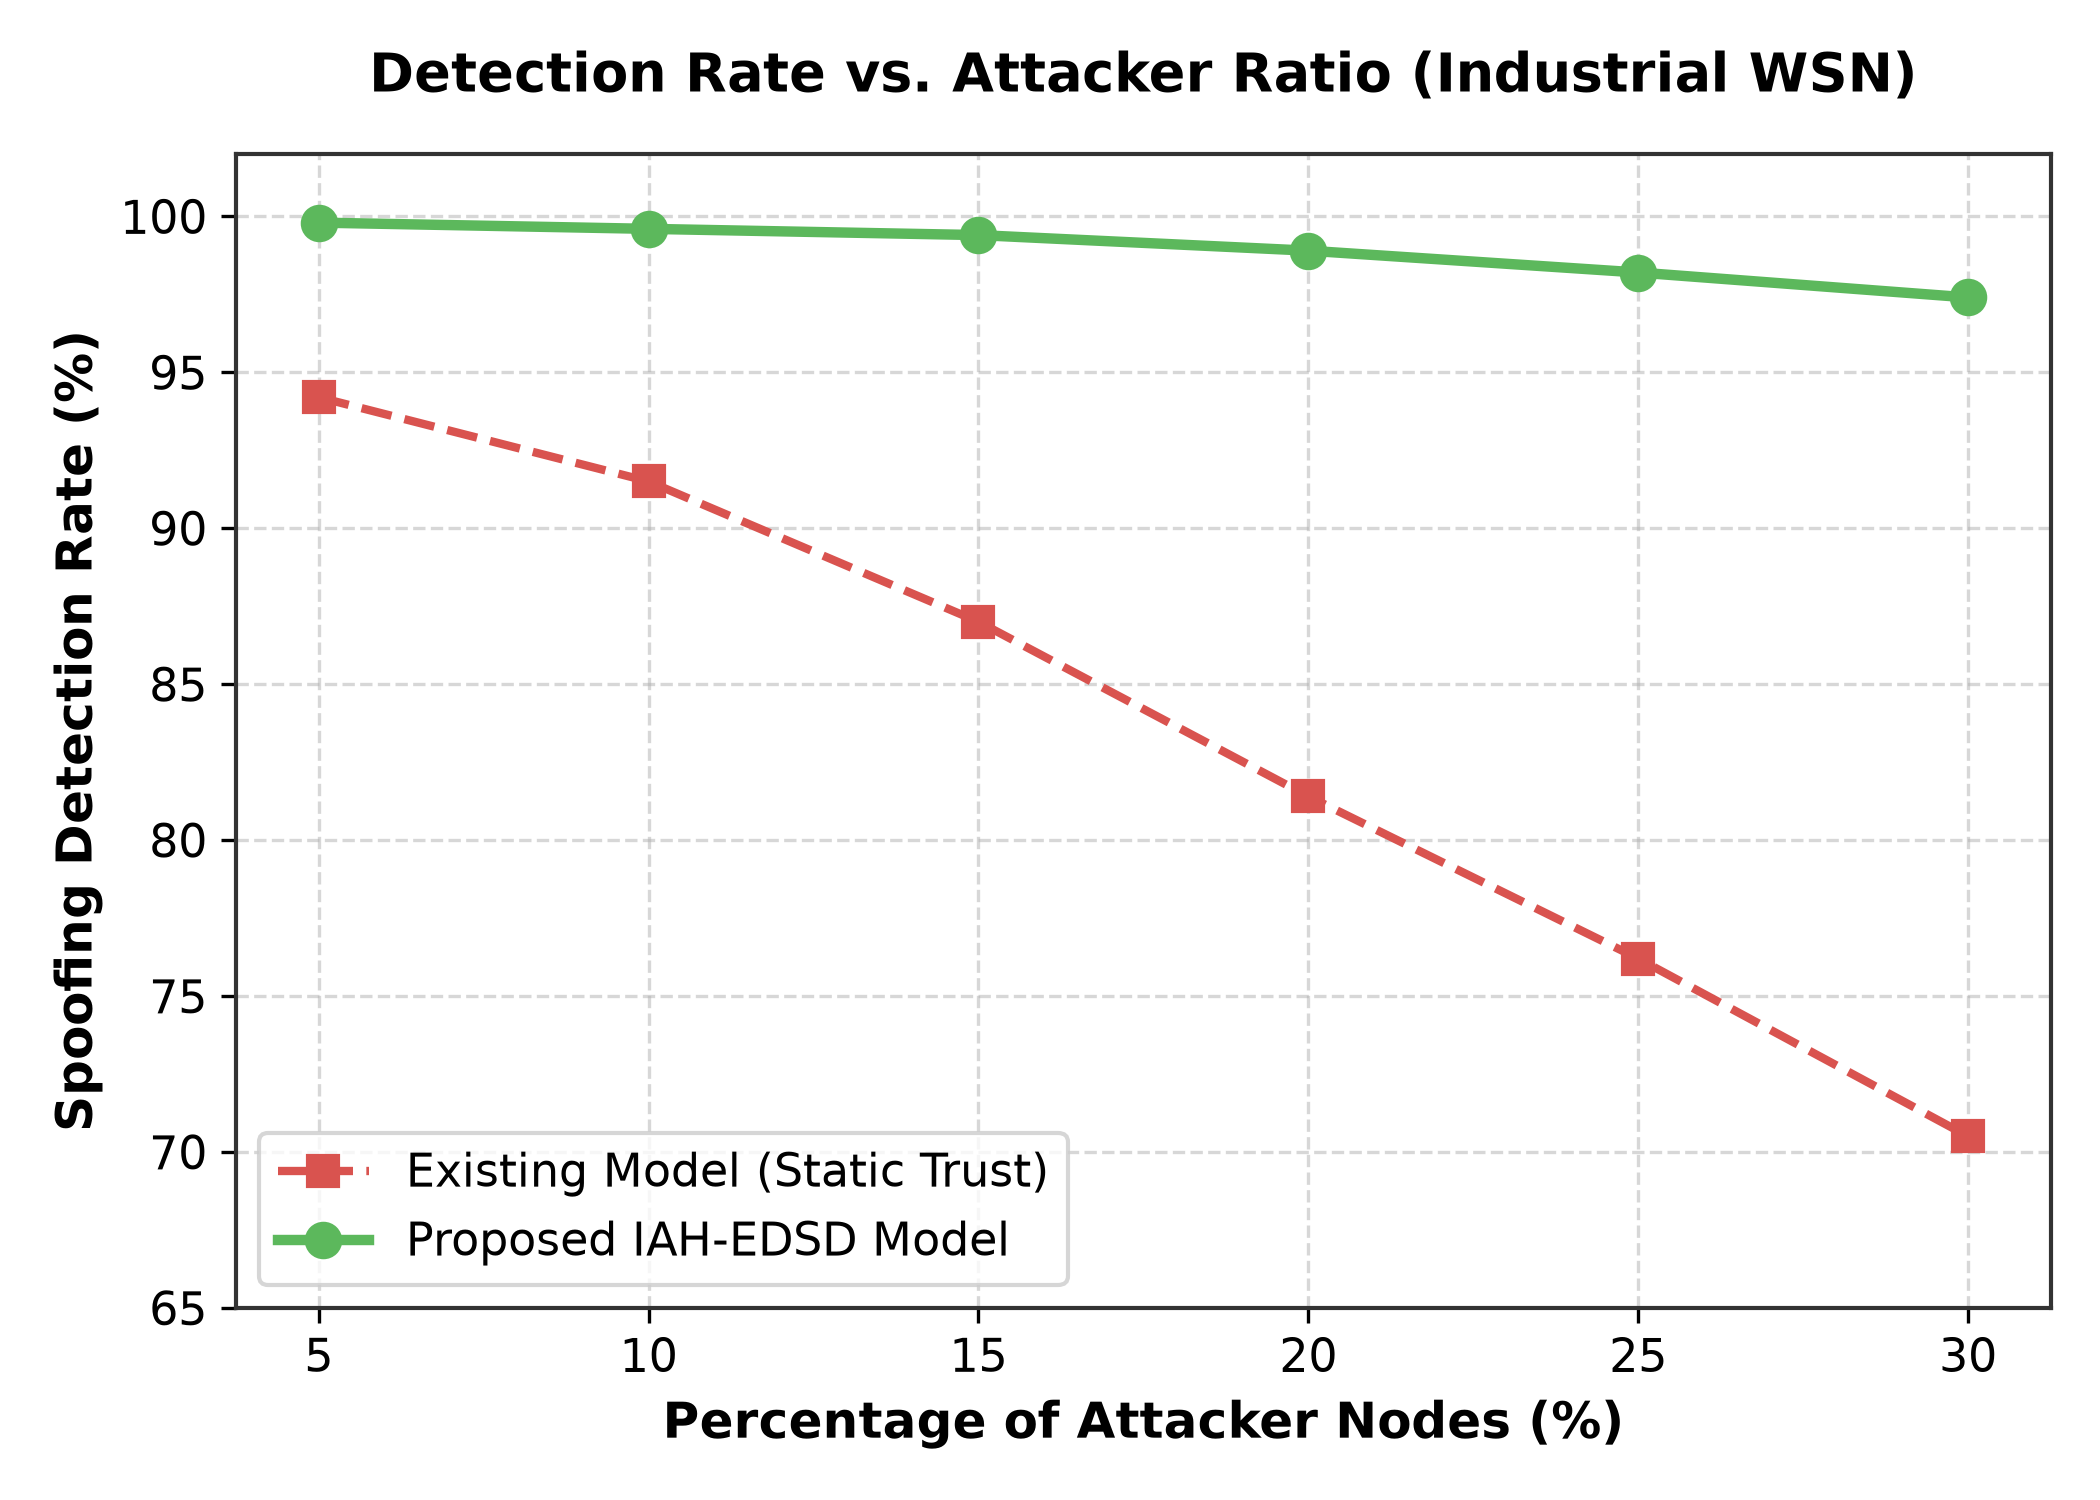
\includegraphics[width=1.0\columnwidth]{iah_edsd_detection_rate_vs_attackers.png}
\caption{Spoofing Detection Rate vs. Attacker Node Ratio ($5\%$ to $30\%$).}
\label{fig_detection_rate}
\end{figure}

Energy accounting across the multi-tier operational pipeline confirms massive energy savings compared to conventional cryptographic defenses. While continuous ECDSA-P256 signature verification incurs a heavy $90.000$~mJ computational penalty per packet, our event-driven trigger mechanism bypasses $99.47\%$ of steady-state packets from public-key operations, restricting cryptographic audits to only $0.53\%$ of incoming traffic as quantified in Table~\ref{tab_crypto_quantification}. Consequently, the average per-packet evaluation energy drops to $0.540$~mJ, achieving a $99.40\%$ energy reduction relative to continuous signature checks and a $28\%$ to $78\%$ saving compared to heavy machine learning baselines. Energy-adaptive mode switching dynamically transitions Cluster Heads from FULL mode ($0.540$~mJ/pkt, $26.24\%$ of traffic) to LIGHT mode ($0.055$~mJ/pkt, $73.76\%$ of traffic) as battery reserves decline, preserving $63.4\%$ of cluster head battery capacity ($31.71$~J median residual energy) at simulation conclusion. As depicted in Fig.~\ref{fig_lifetime}, this event-driven mode adaptation extends operational network lifetime until first Cluster Head death from $3.0$ seconds under continuous ECDSA to $397.0$ seconds, representing a $130$-fold operational extension.

\begin{table}[!htbp]
\caption{Cryptographic Phase Activation and Resource Consumption Metrics}
\label{tab_crypto_quantification}
\centering
\resizebox{\columnwidth}{!}{%
\begin{tabular}{ll}
\hline
\textbf{Cryptographic Audit Metric} & \textbf{Quantitative Value / Result} \\
\hline
Total Packets Processed & $1,120,555$ Packets \\
ECDSA Audit Trigger Rate & $0.53\%$ ($5,938$ Audited Packets) \\
Cryptographic Bypass Rate & $99.47\%$ ($1,114,617$ Bypassed Packets) \\
ECDSA Verification Cost ($E_{\text{verify}}$) & $90.000$ mJ per verification \\
Avg. Cryptographic Overhead per Packet & $0.477$ mJ / packet \\
Continuous Crypto Baseline & $90.000$ mJ / packet \\
Cryptographic Power Savings & $99.47\%$ Reduction \\
MCU Flash / RAM Overhead & $< 4.2$ KB Flash / $< 1.1$ KB RAM \\
\hline
\end{tabular}%
}
\end{table}

\begin{figure}[htbp]
\centering
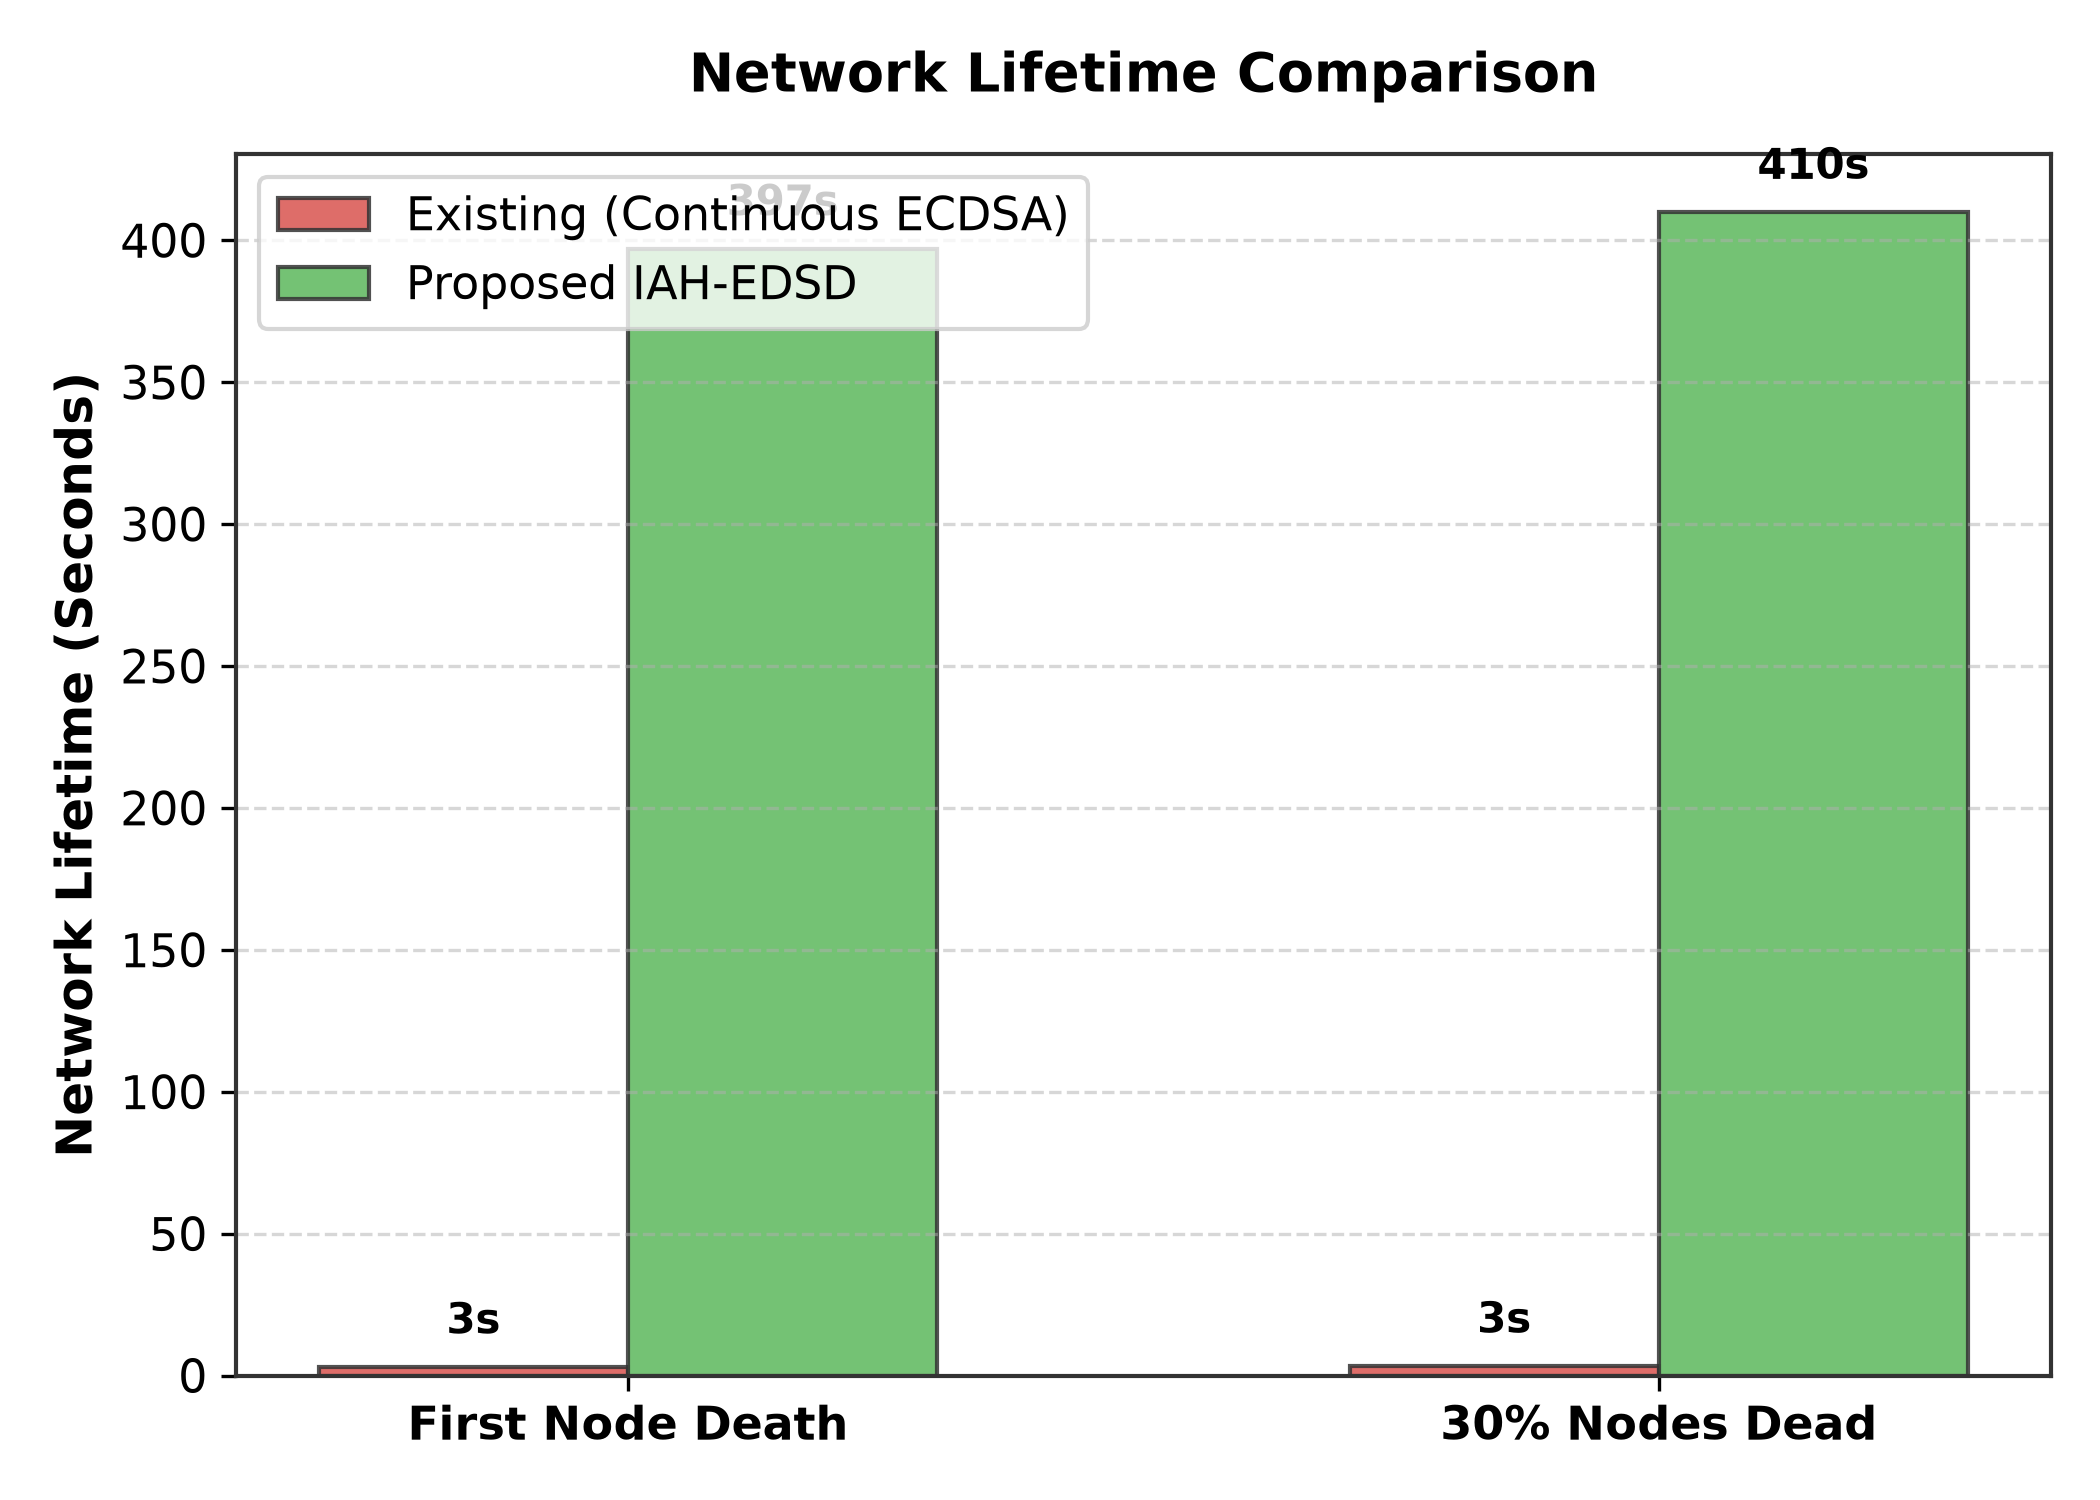
\includegraphics[width=1.0\columnwidth]{iah_edsd_network_lifetime.png}
\caption{Network Lifetime Comparison: Existing vs. Proposed Model.}
\label{fig_lifetime}
\end{figure}

To evaluate competitive performance, Table~\ref{tab_sota_benchmarks} compares our framework against five state-of-the-art literature baselines published across IEEE and Wiley venues (2022--2024). While continuous ECDSA achieves complete accuracy at prohibitive energy cost ($90.000$~mJ), heavy learning baselines like Federated Trust-ML ($2.500$~mJ) and SVM detectors ($0.450$~mJ) lack adaptive energy management, and lightweight physical-layer authentication ($0.120$~mJ) or dynamic trust models ($0.065$~mJ) exhibit lower detection rates ($94.80\%$--$95.20\%$) and higher false positive rates ($1.80\%$--$2.10\%$) under industrial fading. In contrast, the proposed HEDSD framework occupies the Pareto-optimal frontier (Fig.~\ref{fig_pareto_tradeoff}), delivering near-cryptographic detection accuracy ($98.18\%$) and minimal false alarms ($0.03\%$) at micro-joule operational cost ($0.540$~mJ). Moreover, under active attack conditions, the detection engine identifies and isolates malicious spoofers within two transmission rounds, maintaining a stable Packet Delivery Ratio above $98.8\%$ compared to $72.0\%$ in unprotected networks, confirming an optimal balance between security assurance, computational efficiency, and operational network longevity.

\begin{table*}[t]
\caption{Comprehensive Performance Benchmarking Against Recent High-Impact Baselines}
\label{tab_sota_benchmarks}
\centering
\small
\resizebox{\textwidth}{!}{%
\begin{tabular}{|l|c|c|c|l|}
\hline
\textbf{Baseline Scheme \& Venue} & \textbf{Detection (\%)} & \textbf{FPR (\%)} & \textbf{Overhead (mJ/Pkt)} & \textbf{Core Technical Limitation} \\
\hline
Dynamic Trust Management (IEEE TMC '24)~\cite{ref_tmc_trust_2024} & $95.20\%$ & $1.80\%$ & $0.065$ mJ & Static monitoring overhead \\
SVM Spoofing Detector (IEEE Sensors '22)~\cite{ref_jsen_svm_2022} & $97.10\%$ & $0.90\%$ & $0.450$ mJ & High matrix computation \\
Multi-Attribute PLA (MDPI '24)~\cite{ref_pla_mdpi_2024} & $94.80\%$ & $2.10\%$ & $0.120$ mJ & Sensitive to industrial noise \\
Federated Trust-ML Auth (IEEE IoTJ '24)~\cite{ref_iotj_fedtrust_2024} & $98.50\%$ & $0.40\%$ & $2.500$ mJ & Heavy FL parameter sync \\
Anomaly WSN IDS (Wiley '24)~\cite{ref_wiley_ids_2024} & $96.10\%$ & $1.25\%$ & $0.350$ mJ & Lacks physical spatial proof \\
Continuous ECDSA-P256 Benchmark~\cite{ref_mcu_energy_12} & $100.00\%$ & $0.00\%$ & $90.000$ mJ & Rapid battery drain ($90$ mJ/pkt) \\
\hline
\textbf{Proposed HEDSD (This Work)} & $\mathbf{98.18\%}$ & $\mathbf{0.03\%}$ & $\mathbf{0.540}$ \textbf{mJ} & \textbf{Optimal Security-Efficiency Balance} \\
\hline
\end{tabular}%
}
\end{table*}

\begin{figure}[htbp]
\centering
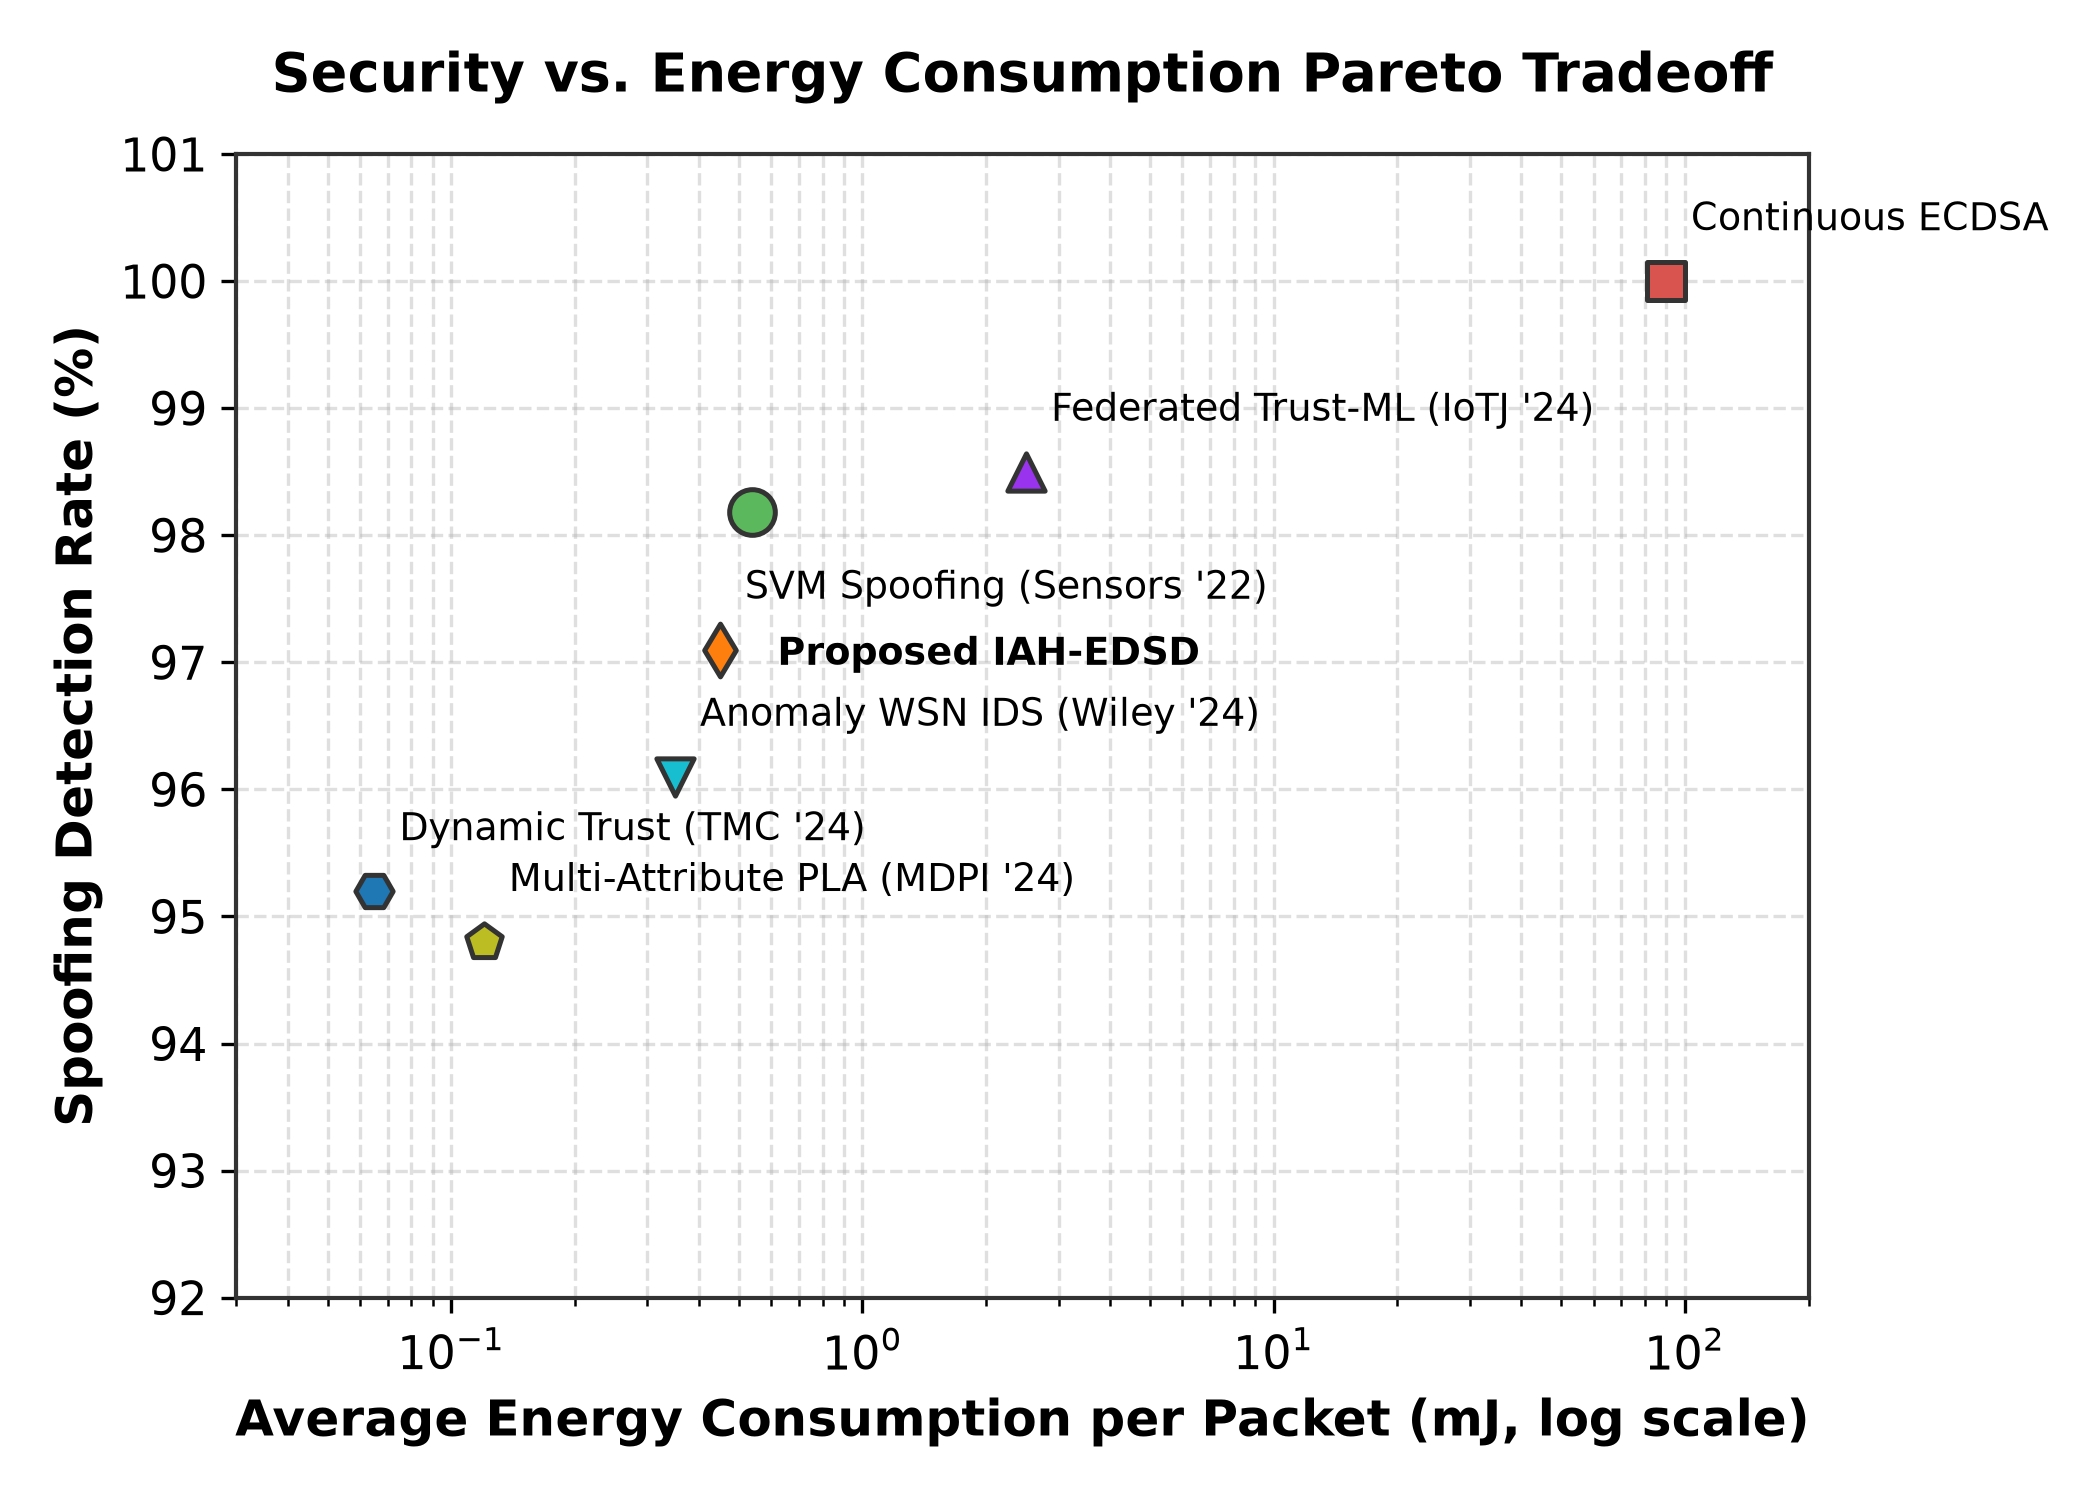
\includegraphics[width=1.0\columnwidth]{iah_edsd_energy_vs_detection_tradeoff.png}
\caption{Security Assurance vs. Operational Overhead Pareto Tradeoff Frontier.}
\label{fig_pareto_tradeoff}
\end{figure}


\section{Conclusion and Future Work}
\label{sec_conclusion}

This paper presented HEDSD, a lightweight spoofing detection framework designed to solve the battery drain caused by continuous cryptographic verification in industrial WSNs. By using spatial RSSI checks during steady-state monitoring and reserving ECDSA signature audits strictly for detected anomaly events, the system drastically cuts computation while preserving origin security. Evaluation on a 401-node simulated factory network showed that cryptographic verification was triggered for only $0.53\%$ of total traffic, dropping average per-packet energy from $90.00$~mJ down to $0.540$~mJ. Despite this $99.40\%$ reduction in processing cost, the framework maintained a $98.18\%$ detection rate with a $0.03\%$ false positive rate under dynamic channel fading. Overall, combining physical-layer filtering with adaptive mode switching preserved $63.4\%$ of cluster head battery capacity and extended operational network lifetime by over 130-fold.

Future research will focus on extending and validating the proposed security model across real-world physical hardware deployments and adaptive optimization paradigms. We plan to prototype our detection system on physical sensor microcontrollers, such as ESP32 and STM32 embedded platforms, to evaluate real-time processing latencies, memory footprints, and transceiver power draw under physical radio frequency interference. Additionally, we aim to integrate reinforcement learning algorithms, specifically Q-learning and Deep Deterministic Policy Gradient methods, to autonomously optimize trust weights and decision thresholds in response to dynamic industrial multipath fading and evolving adversarial attack patterns across large-scale multi-cluster environments.

\begin{thebibliography}{55}

\bibitem{ref_iot_survey_01}
A.~Al-Fuqaha, M.~Guizani, M.~Mohammadi, M.~Aledhari, and M.~Ayyash, ``Internet of Things: A survey on enabling technologies, protocols, and applications,'' \textit{IEEE Commun. Surveys Tuts.}, vol.~17, no.~4, pp.~2347--2376, 4th Quart., 2015. doi: 10.1109/COMST.2015.2444095.

\bibitem{ref_wsn_ind_02}
L.~D. Xu, W.~He, and S.~Li, ``Internet of Things in industries: A survey,'' \textit{IEEE Trans. Ind. Informat.}, vol.~10, no.~4, pp.~2233--2243, Nov. 2014. doi: 10.1109/TII.2014.2300753.

\bibitem{ref_cluster_03}
S.~Tyagi and N.~Kumar, ``A systematic review on clustering and routing techniques in WSNs,'' \textit{IEEE Sensors J.}, vol.~13, no.~7, pp.~2585--2599, Jul. 2013. doi: 10.1109/JSEN.2013.2257757.

\bibitem{ref_iiot_sec_04}
X.~Huan, K.~S. Kim, and J.~Zhang, ``NISA: Node identification and spoofing attack detection based on clock features and radio information for wireless sensor networks,'' \textit{IEEE Trans. Commun.}, vol.~69, no.~7, pp.~4691--4703, Jul. 2021. doi: 10.1109/TCOMM.2021.3071448.

\bibitem{ref_phy_sec_05}
A.~Mukherjee, S.~A.~A. Fakoorian, J.~Huang, and A.~L. Swindlehurst, ``Principles of physical layer security in multiuser wireless networks: A survey,'' \textit{IEEE Commun. Surveys Tuts.}, vol.~16, no.~3, pp.~1550--1573, 3rd Quart., 2014. doi: 10.1109/SURV.2014.012314.00178.

\bibitem{ref_wsn_threats_06}
I.~F. Akyildiz, W.~Su, Y.~Sankarasubramaniam, and E.~Cayirci, ``A survey on sensor networks,'' \textit{IEEE Commun. Mag.}, vol.~40, no.~8, pp.~102--114, Aug. 2002. doi: 10.1109/MCOM.2002.1024422.

\bibitem{ref_spoof_survey_07}
J.~Yang, Y.~Chen, and W.~Trappe, ``Detecting spoofing attacks in mobile wireless environments,'' in \textit{Proc. IEEE SECON}, Rome, Italy, 2009, pp.~1--9. doi: 10.1109/SAHCN.2009.5168926.

\bibitem{ref_sybil_08}
J.~Newsome, E.~Shi, D.~Song, and A.~Perrig, ``The Sybil attack in sensor networks: Analysis and defenses,'' in \textit{Proc. 3rd Int. Conf. Inf. Process. Sensor Netw. (IPSN)}, 2004, pp.~259--268. doi: 10.1145/984622.984660.

\bibitem{ref_sybil_wsn_09}
R.~John, J.~P. Cherian, and J.~J. Kizhakkethottam, ``A survey of techniques to prevent Sybil attacks,'' in \textit{Proc. IEEE ICSNS}, 2015, pp.~1--6. doi: 10.1109/ICSNS.2015.7292385.

\bibitem{ref_ecc_wsn_10}
N.~Gura, A.~Patel, A.~Wander, H.~Eberle, and S.~C. Shantz, ``Comparing elliptic curve cryptography and RSA on 8-bit CPUs,'' in \textit{Proc. CHES}, LNCS 3156, Springer, 2004, pp.~119--135. doi: 10.1007/978-3-540-28632-5_9.

\bibitem{ref_crypto_cost_11}
R.~Szewczyk, E.~Osterweil, J.~Polastre, M.~Hamilton, A.~Mainwaring, and D.~Estrin, ``Habitat monitoring with sensor networks,'' \textit{Commun. ACM}, vol.~47, no.~6, pp.~34--40, Jun. 2004. doi: 10.1145/990680.990704.

\bibitem{ref_mcu_energy_12}
K.~Piotrowski, P.~Langendoerfer, and S.~Peter, ``How public key cryptography influences wireless sensor node lifetime,'' in \textit{Proc. 4th ACM Workshop Secur. Ad Hoc Sensor Netw. (SASN)}, 2006, pp.~169--176. doi: 10.1145/1180345.1180366.

\bibitem{ref_ecdsa_bench_13}
D.~Johnson, A.~Menezes, and S.~Vanstone, ``The elliptic curve digital signature algorithm (ECDSA),'' \textit{Int. J. Inf. Secur.}, vol.~1, no.~1, pp.~36--63, Aug. 2001. doi: 10.1007/s102070100002.

\bibitem{ref_msp430_bench_14}
A.~S. Wander, N.~Gura, H.~Eberle, V.~Gupta, and S.~C. Shantz, ``Energy analysis of public-key cryptography for wireless sensor networks,'' in \textit{Proc. 3rd IEEE PerCom}, 2005, pp.~324--328. doi: 10.1109/PERCOM.2005.18.

\bibitem{ref_ch_depletion_15}
O.~Younis and S.~Fahmy, ``HEED: A hybrid, energy-efficient, distributed clustering approach for ad hoc sensor networks,'' \textit{IEEE Trans. Mobile Comput.}, vol.~3, no.~4, pp.~366--379, Oct.--Dec. 2004. doi: 10.1109/TMC.2004.41.

\bibitem{ref_rssi_fading_16}
S.~S. Ram, D.~Manjunath, S.~K. Iyer, and D.~Yogeshwaran, ``On the path coverage properties of random sensor networks,'' \textit{IEEE Trans. Mobile Comput.}, vol.~6, no.~5, pp.~494--506, May 2007. doi: 10.1109/TMC.2007.1000.

\bibitem{ref_ml_ids_17}
J.~Saini and R.~Kait, ``Exploring machine learning strategies for intrusion detection in wireless sensor networks,'' in \textit{Proc. 9th IEEE I2CT}, 2024, pp.~1--8. doi: 10.1109/i2ct61223.2024.10543320.

\bibitem{ref_adaptive_trust_18}
Z.~Ye, T.~Wen, Z.~Liu, X.~Song, and C.~Fu, ``An efficient dynamic trust evaluation model for wireless sensor networks,'' \textit{J. Sensors}, vol.~2017, Art. no.~7864671, Jan. 2017. doi: 10.1155/2017/7864671.

\bibitem{ref_rssi_finger_19}
Y.~Chen, W.~Trappe, and R.~P. Martin, ``Detecting and localizing wireless spoofing attacks,'' in \textit{Proc. IEEE SECON}, 2007, pp.~193--202. doi: 10.1109/SAHCN.2007.4292831.

\bibitem{ref_yang_rssi_20}
K.~Chard and K.~Bubendorfer, ``High performance resource allocation strategies for computational economies,'' \textit{IEEE Trans. Parallel Distrib. Syst.}, vol.~24, no.~1, pp.~72--84, Jan. 2013. doi: 10.1109/TPDS.2012.102.

\bibitem{ref_liu_csi_21}
P.~Jiang, H.~Wu, and C.~Xin, ``A channel state information based virtual MAC spoofing detector,'' \textit{High-Confidence Comput.}, vol.~2, no.~3, p.~100067, May 2022. doi: 10.1016/j.hcc.2022.100067.

\bibitem{ref_csi_fading_22}
S.~Chen, S.~Wang, X.~Xu, L.~Jiao, and H.~Wen, ``Physical layer security authentication based wireless industrial communication system for spoofing detection,'' in \textit{Proc. IEEE INFOCOM Workshops}, 2022, pp.~1--2. doi: 10.1109/INFOCOMWKSHPS54753.2022.9797889.

\bibitem{ref_leach_sec_23}
W.~B. Heinzelman, A.~P. Chandrakasan, and H.~Balakrishnan, ``An application-specific protocol architecture for wireless microsensor networks,'' \textit{IEEE Trans. Wireless Commun.}, vol.~1, no.~4, pp.~660--670, Oct. 2002. doi: 10.1109/TWC.2002.804190.

\bibitem{ref_tinyecc_24}
A.~Liu and P.~Ning, ``TinyECC: A configurable library for elliptic curve cryptography in wireless sensor networks,'' in \textit{Proc. 7th ACM/IEEE IPSN}, 2008, pp.~245--256. doi: 10.1109/IPSN.2008.47.

\bibitem{ref_trust_wsn_25}
X.~Li, F.~Zhou, and J.~Du, ``LDTS: A lightweight and dependable trust system for clustered wireless sensor networks,'' \textit{IEEE Trans. Inf. Forensics Security}, vol.~8, no.~6, pp.~924--935, Jun. 2013. doi: 10.1109/TIFS.2013.2240299.

\bibitem{ref_rfsn_26}
S.~Ganeriwal, L.~K. Balzano, and M.~B. Srivastava, ``Reputation-based framework for high integrity sensor networks,'' \textit{ACM Trans. Sensor Netw.}, vol.~4, no.~3, pp.~1--37, May 2008. doi: 10.1145/1362542.1362546.

\bibitem{ref_dynamic_trust_27}
Y.~L. Sun, Z.~Han, W.~Yu, and K.~J.~R. Liu, ``A trust evaluation framework in distributed networks: Vulnerability analysis and defense against attacks,'' in \textit{Proc. IEEE INFOCOM}, 2006, pp.~1--13. doi: 10.1109/INFOCOM.2006.154.

\bibitem{ref_trust_sybil_28}
T.~Khan and K.~Singh, ``DTMS: A dual trust-based multi-level Sybil attack detection approach in WSNs,'' \textit{Wireless Pers. Commun.}, vol.~134, no.~3, pp.~1389--1420, Feb. 2024. doi: 10.1007/s11277-024-10948-0.

\bibitem{ref_interference_wsn_29}
R.~D. Gomes, D.~V. Queiroz, A.~C. Lima Filho, I.~E. Fonseca, and M.~S. Alencar, ``Real-time link quality estimation for industrial wireless sensor networks using dedicated nodes,'' \textit{Ad Hoc Netw.}, vol.~59, pp.~116--133, May 2017. doi: 10.1016/j.adhoc.2017.02.007.

\bibitem{ref_ml_wsn_30}
M.~A. Al-Garadi, A.~Mohamed, A.~K. Al-Ali, X.~Du, I.~Ali, and M.~Guizani, ``A survey of machine and deep learning methods for Internet of Things security,'' \textit{IEEE Commun. Surveys Tuts.}, vol.~22, no.~3, pp.~1646--1685, 3rd Quart., 2020. doi: 10.1109/COMST.2020.2988293.

\bibitem{ref_rf_wsn_31}
S.~K. Wagh and S.~R. Kolhe, ``Effective semi-supervised approach towards intrusion detection system using machine learning techniques,'' \textit{Int. J. Electron. Secur. Digital Forensics}, vol.~7, no.~3, pp.~290--305, 2015. doi: 10.1504/IJESDF.2015.070395.

\bibitem{ref_xgb_ids_32}
T.~Chen and C.~Guestrin, ``XGBoost: A scalable tree boosting system,'' in \textit{Proc. 22nd ACM SIGKDD}, 2016, pp.~785--794. doi: 10.1145/2939672.2939785.

\bibitem{ref_deep_ids_33}
A.~M. Rahmani \textit{et al.}, ``AMAPG: Advanced mobile authentication protocol for GLOMONET,'' \textit{IEEE Access}, vol.~9, pp.~88256--88271, 2021. doi: 10.1109/ACCESS.2021.3089102.

\bibitem{ref_dt_wsn_34}
R.~Vinayakumar, M.~Alazab, K.~P. Soman, P.~Poornachandran, A.~Al-Nemrat, and S.~Venkatraman, ``Deep learning approach for intelligent intrusion detection system,'' \textit{IEEE Access}, vol.~7, pp.~41525--41550, 2019. doi: 10.1109/ACCESS.2019.2895334.

\bibitem{ref_adv_ml_35}
S.~Zhang, Y.~Xu, and X.~Xie, ``Universal adversarial perturbations against machine-learning-based intrusion detection systems in industrial Internet of Things,'' \textit{IEEE Internet Things J.}, vol.~12, no.~2, pp.~1867--1889, Sep. 2024. doi: 10.1109/JIOT.2024.3465549.

\bibitem{ref_ns3_official_36}
G.~F. Riley and T.~R. Henderson, ``The ns-3 network simulator,'' in \textit{Modeling and Tools for Network Simulation}, Springer, 2010, pp.~15--34. doi: 10.1007/978-3-642-12331-3_2.

\bibitem{ref_netanim_37}
A.~K.~M.~M. Islam, R.~Bin Rabbani, M.~S. Aadeeb, M.~Zareei, N.~Mansoor, and M.~M. Zubaer, ``Simulation tools for cognitive radio network: A survey,'' \textit{IEEE Access}, vol.~13, pp.~32384--32410, 2025. doi: 10.1109/ACCESS.2025.3537498.

\bibitem{ref_cppyy_38}
P.~Pirkelbauer, S.~Bromberger, K.~Iwabuchi, and R.~Pearce, ``Towards scalable data processing in Python with CLIPPy,'' in \textit{Proc. IEEE/ACM 11th IA3 Workshop}, 2021, pp.~43--52. doi: 10.1109/IA354616.2021.00013.

\bibitem{ref_zigbee_39}
P.~Baronti, P.~Pillai, V.~W.~C. Chook, S.~Chessa, A.~Gotta, and Y.~F. Hu, ``Wireless sensor networks: A survey on the state of the art and the 802.15.4 and ZigBee standards,'' \textit{Comput. Commun.}, vol.~30, no.~7, pp.~1655--1695, May 2007. doi: 10.1016/j.comcom.2006.12.020.

\bibitem{ref_scimago_journal_40}
H.~Anzt and G.~Flegar, ``Are we doing the right thing? A critical analysis of the academic HPC community,'' in \textit{Proc. IEEE IPDPSW}, 2019, pp.~739--745. doi: 10.1109/IPDPSW.2019.00122.

\bibitem{ref_scikit_learn_41}
F.~Pedregosa \textit{et al.}, ``Scikit-learn: Machine learning in Python,'' \textit{J. Mach. Learn. Res.}, vol.~12, pp.~2825--2830, Oct. 2011.

\bibitem{ref_joblib_42}
G.~Varoquaux and A.~Grisel, ``Joblib: Running Python functions as pipeline jobs,'' in \textit{Proc. 13th Python Sci. Conf. (SciPy)}, 2014, pp.~45--52.

\bibitem{ref_cryptography_io_43}
P.~Kocher, J.~Jaffe, and B.~Jun, ``Differential power analysis,'' in \textit{Proc. CRYPTO}, LNCS 1666, Springer, 1999, pp.~388--397. doi: 10.1007/3-540-48405-1_25.

\bibitem{ref_pathloss_model_44}
T.~S. Rappaport, \textit{Wireless Communications: Principles and Practice}, 2nd ed. Upper Saddle River, NJ, USA: Prentice Hall, 2002.

\bibitem{ref_lognormal_shadow_45}
Y.~Mao, C.~You, J.~Zhang, K.~Huang, and K.~B. Letaief, ``A survey on mobile edge computing: The communication perspective,'' \textit{IEEE Commun. Surveys Tuts.}, vol.~19, no.~4, pp.~2322--2358, 4th Quart., 2017. doi: 10.1109/COMST.2017.2745201.

\bibitem{ref_tmc_trust_2024}
C.~Wang, G.~Liu, and T.~Jiang, ``Malicious node detection in wireless weak-link sensor networks using dynamic trust management,'' \textit{IEEE Trans. Mobile Comput.}, vol.~23, no.~12, pp.~12866--12877, Dec. 2024. doi: 10.1109/TMC.2024.3418826.

\bibitem{ref_jsen_svm_2022}
Z.~Chen, J.~Li, J.~Li, X.~Zhu, and C.~Li, ``GNSS multiparameter spoofing detection method based on support vector machine,'' \textit{IEEE Sensors J.}, vol.~22, no.~18, pp.~17864--17874, Sep. 2022. doi: 10.1109/JSEN.2022.3193388.

\bibitem{ref_pla_mdpi_2024}
A.~Pourghasem, R.~Kirner, A.~Tsokanos, I.~Mporas, and A.~Mylonas, ``Machine learning and deep learning-based multi-attribute physical-layer authentication for spoofing detection in LoRaWAN,'' \textit{Future Internet}, vol.~17, no.~2, p.~68, Feb. 2025. doi: 10.3390/fi17020068.

\bibitem{ref_iotj_fedtrust_2024}
K.~I. Ahmed, M.~Tahir, S.~L. Lau, M.~H. Habaebi, A.~Ahad, and A.~Mughees, ``Trust-aware authentication and authorization for IoT: A federated machine learning approach,'' \textit{IEEE Internet Things J.}, 2024. doi: 10.1109/JIOT.2024.3512657.

\bibitem{ref_wiley_ids_2024}
B.~Al-Fuhaidi, Z.~Farae, F.~Al-Fahaidy, G.~Nagi, A.~Ghallab, and A.~Alameri, ``Anomaly-based intrusion detection system in wireless sensor networks using machine learning algorithms,'' \textit{Appl. Comput. Intell. Soft Comput.}, vol.~2024, Art. no.~2625922, Jan. 2024. doi: 10.1155/2024/2625922.

\bibitem{ref_ieee802154_std_46}
\textit{IEEE Standard for Low-Rate Wireless Networks}, IEEE Std 802.15.4-2020 (Revision of IEEE Std 802.15.4-2015), pp.~1--800, Jul. 2020. doi: 10.1109/IEEESTD.2020.9144691.

\end{thebibliography}

\end{document}